\section{Identification of wave spectrum model}
\subsection{Power spectral density estimate}
The Power Spectral Density function is the autocorrelation function expressed in the frequency domain. It is formally defined as the Fourier Transform of the autocorrelation function.  The MATLAB function \texttt{pwelch} calculates an estimate of the power spectral density PSD through
dividing the signal into K overlapping blocks multiplied by a windowing function, and finding the periodogram of each one.  The result of sending the waves disturbance, $\psi_w$, through \texttt{pwelch} is shown in \cref{fig:2a-welchPSDestimate}.

\begin{figure}[h]
    \centering
    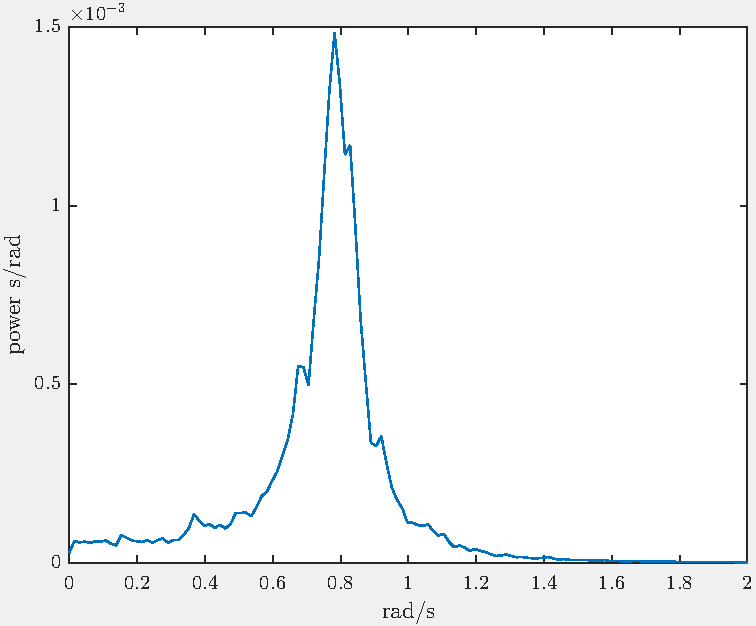
\includegraphics[width=0.5\textwidth]{images/2a-welchPSDestimate}
    \caption{Welch PSD estimate}
    \label{fig:2a-welchPSDestimate}
\end{figure}

\subsection{Expression for $P_{\Psi_{w}}$ and $H_{\Psi_{w}}$}
Using the following state equations in the problem description \cite{assignment}

\begin{align*}
    \xi_w &= \psi_w \\
    \dot{\psi}_w &= -\omega^2_0\xi_w - 2\lambda\omega_0\psi_w + K_ww_w
\end{align*}

the transfer function between $w_w$ and $\psi_w$ can be found.

Replacing $\xi_w$ with $\int\psi_w$ and taking the Laplace transform leads to:
\begin{align*}
    \Psi_w(s)s &= -\omega^2_0\Psi_w(s)\frac{1}{s} - 2\lambda\omega_0\Psi_w(s) + K_ww_w(s)
\end{align*}

Rearrange terms to get the transfer function:
\begin{align*}
    \frac{\Psi_w(s)}{w_w(s)} &= \frac{K_ws}{s^2 + 2\lambda\omega_0s + \omega^2_0}
\end{align*}

The autocorrelation of a random signal given stationarity is the following:
\begin{equation*}
R_{\siw}(\tau) = E(\siw(t)\siw(t-\tau))
\end{equation*}

The Power Spectral Density function (PSD) of a random signal is the Fourier transform of the autocorrelation of that signal.

\begin{equation*}
    S_{\siw}(j\omega) = \mathcal{F}[R_{\siw}(\tau)] = \int_{-\infty}^{\infty}R_{\siw}(\tau)e^{-j\omega\tau}d\tau
\end{equation*}

To find the Power Density Spectrum (PSD) of $\Psi_w$, we use the following relation \cite{brown12}:
\begin{equation*}
S_y(j\omega) = |H(j\omega)|^2S_x(j\omega)
\end{equation*}
Where $y$ is the output, $x$ is the input, and $H$ is the Fourier transfer function between them. Because $w_w$ is white noise, it has PSD $S_{w_w} = \sigma_{w_w}^2$. Here, $\Psi_{w_w}$ is the output, $w_w$ is the input, and $\frac{\Psi_w(s)}{w_w(s)}$ is the transfer function between them. Here we use the relation between the Laplace and the Fourier transform where $\mathcal{F}(X(t))(j\omega) = \mathcal{L}(X(t))(s)\bigg{|}_{s=j\omega}$ in order to find the Fourier transform as $\frac{\Psi_w(s)}{w_w(s)}\bigg{|}_{s=j\omega}$. The PSD is thus:

\begin{align*}
P_{\Psi_w}(\omega) &= |\frac{\Psi_w(s)}{w_w(s)}|^2\bigg{|}_{s=j\omega}S_{w_w} \\
&= \frac{|K_ws|^2}{|s^2 + 2\lambda\omega_0s + \omega^2_0|}\bigg{|}_{s=j\omega}\sigma_{w_w}^2
\end{align*}
Where $\sigma_{w_w}^2$ equals to one, because $w_w$ is zero mean white noise with unity variance.
\begin{align*}
    P_{\Psi_w}(\omega) &= \frac{|K_ws|^2}{|s^2 + 2\lambda\omega_0s + \omega^2_0|}\bigg{|}_{s=j\omega} \\ &= K_w^2\frac{\omega^2}{\left|-\omega^2+\omega^2_0+2\lambda\omega_0\omega\right|^2} \\
    &= \frac{K_w^2w^2}{w^4+(4\lambda^2-2)w_0^2w^2+w_0^4}
\end{align*}


\subsection{Finding $\omega_0$}
$\omega_0$ is the resonant 
frequency and the point where $\psi_\omega$ correlates the most with itself.  This is the point on the x-axis of \cref{fig:2a-welchPSDestimate} where the y value is largest.
$\omega_0 = 0.7823$, found through finding where the max of pxx$/2\pi$ is in the x-axis. 

\subsection{Identifying $\lambda$ and fitting $P_{\Psi_{w}}$}
$\sigma^2$, the peak value of $P_{\psi_\omega}(\omega)$ is equal to 0.0015.
By setting $K_w = 2\lambda\omega_0\sigma$, the only parameter unknown in $P_{\psi_\omega}(\lambda, \omega)$ is $\lambda$. To fit $\lambda$, the MATLAB function \texttt{lsqcurvefit} was used. It finds $\lambda$ by minimizing the least-squares error
between the target data $S_{\psi_\omega}(\omega)$, and the analytical function $P_{\psi_\omega}(\lambda, \omega)$.
\begin{equation*}
\min_{\lambda}e(\lambda) = \min_{\lambda}(|S_{\psi_\omega}(\omega) - P_{\psi_\omega}(\lambda, \omega)|)^2
\end{equation*}
Where $|S_{\psi_\omega}(\omega) - P_{\psi_\omega}(\lambda, \omega)|$ is the length between the two vectors.

$\lambda$ was found to be 0.0827. The difference between the estimated and analytical PSD functions is shown (\cref{fig:2d-fitted_theoretical_PSD_vs_estimated_PSD}) to be very small.

\begin{figure}[ht]
    \centering
    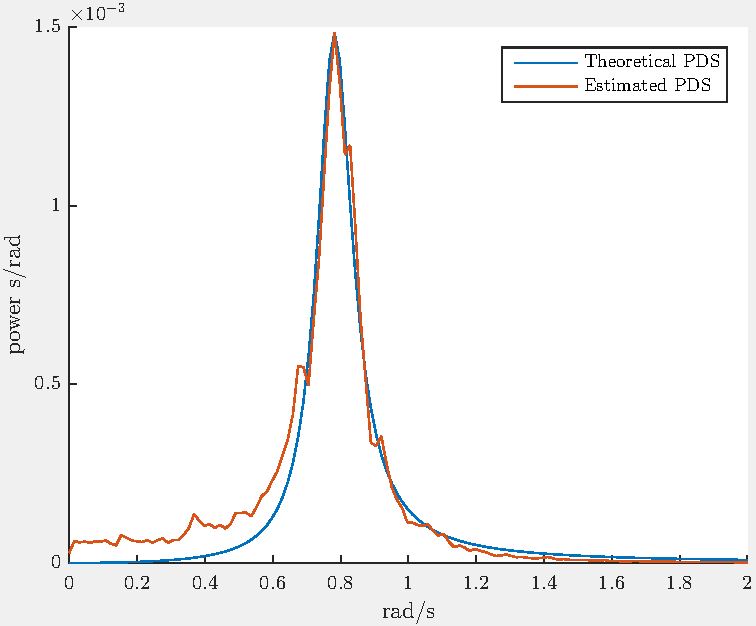
\includegraphics[width=0.5\textwidth]{images/2d-fitted_theoretical_PSD_vs_estimated_PSD}
    \caption{Fitted theoretical PSD vs estimated PSD}
    \label{fig:2d-fitted_theoretical_PSD_vs_estimated_PSD}
\end{figure}
